\section{Build}
\begin{frame}{Prinzip}
 \begin{itemize}
  \item wir sind in \cod{17-build}
  \item pro Komponente ein Skript in \cod{tools}
  \item pro Komponente ein Unterverzeichnis in \cod{build}
  \item der File \cod{tools/common.sh}
  \begin{itemize}
   \item Pfadnamem
  \end{itemize}
 \end{itemize}
\end{frame}

\begin{frame}{Das \target Rootfilesystem}{an zwei Orten}
\begin{center}
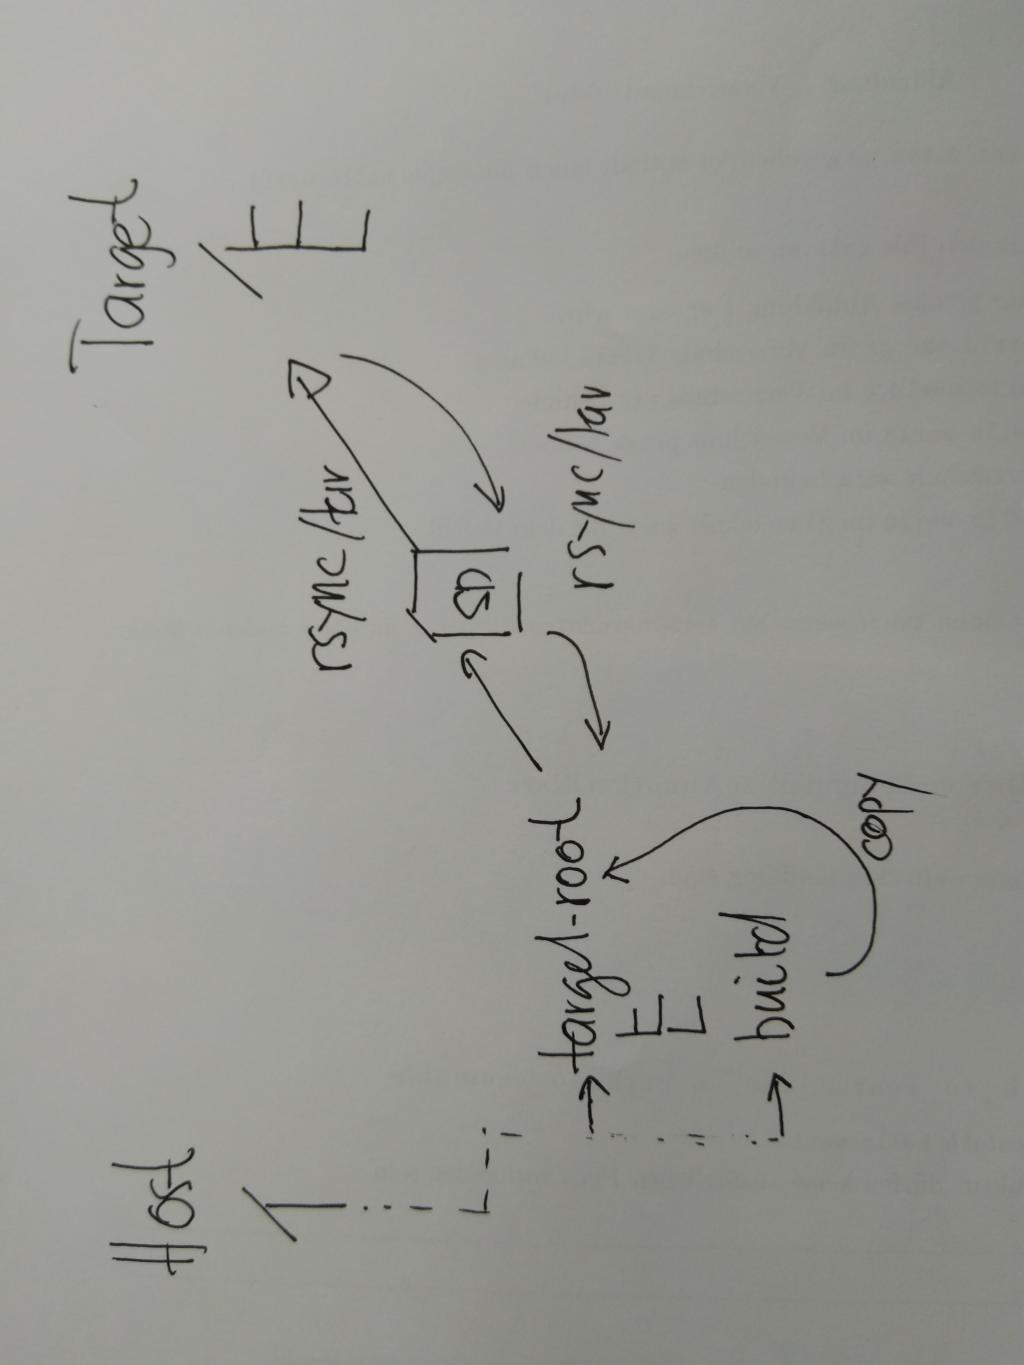
\includegraphics[width=0.5\textwidth,angle=-90]{rootfs.jpg}
\end{center}
\end{frame}

\subsection{Initiales \linux}
\begin{frame}{Build 1}{Toolchain 1}
 \begin{itemize}
  \item \cod{binutils.sh}
  \item \cod{gcc-bare.sh} 
  \begin{itemize}
   \item nur für den {\em kernel}
   \item das bare minimum
   \item nur {\Large C}
  \end{itemize}
 \end{itemize}
\end{frame}

\begin{frame}{Build 2}{Kernel}
 \begin{itemize} 
  \item \cod{kernel.sh} mit ein paar {\em targets}
   \begin{itemize}
    \item \cod{bb.org\_defconfig}
    \item \cod{zImage}
    \item \cod{headers\_install} 
	\begin{itemize}
	 \item Interface: {\em kernel}-{\em libc}
	\end{itemize}
   \end{itemize}
  \end{itemize}
\end{frame}

\begin{frame}{Build 3}{libc}{Wir brauchen glibc}
 \begin{itemize} 
  \item \cod{glibc} 
 \end{itemize}
\end{frame}

\begin{frame}{Build 4}{Toolchain 2}
 \begin{itemize} 
  \item \cod{gcc.sh} 
  \begin{itemize}
   \item mit \cod{sysroot}
   \item {\Large C} und {\Large C++}
  \end{itemize}
  \item Test
  \begin{itemize}\item im Verzeichnis \cod{work}\end{itemize}
 \end{itemize}
\end{frame}

\begin{frame}{Build 5}{busybox}
 \begin{itemize}
  \item \cod{busybox.sh}
  \begin{itemize}
   \item Installation auf SD-Card
   \item \cod{fakeroot}
  \end{itemize}
 \end{itemize}
\end{frame}


\begin{frame}{Skripts und Argumente}{initiales System *) fakultativ}
 \begin{tabular}{l|l|l}
  Skript & target & gebraucht für\\
  \hline\hline
  \cod{binutils.sh}*)& &alles\\
  \hline
  \cod{gcc-bare.sh}*)& &kernel, libc\\
  \hline
  \cod{kernel.sh}*)  & \cod{defconfig}\\
                   & \cod{zImage}\\
                   & \cod{headers\_install}\\
  \hline
  \cod{glibc.sh}  & &POSIX\\
  \hline
  \cod{gcc.sh}*)     & &C/C++, POSIX\\
  \hline
  \cod{busybox.sh} &\cod{menuconfig}\\
  		   &\cod{busybox}\\
  		   &\cod{install}\\
  \hline
  \cod{target-root.sh}&&vervollständigt \cod{target-root}\\
 \end{tabular}
 \remark{Alle Skripte sind {\Large\tt bash} Skripte}
\end{frame}

\begin{frame}{Target}{erster Versuch}
\begin{itemize}
 \item transfer auf SD Karte
 \item Internet
\end{itemize}
\end{frame}

\begin{frame}{Skripts und Argumente}{ssh}
\begin{tabular}{lll}
 \cod{zlib.sh}\\
 \cod{openssl.sh}&&die kryptographischen Algorithmen\\
 \cod{openssh.sh}
\end{tabular}
\remark{\cod{openssh.sh} hängt von \cod{zlib.sh} und \cod{openssl.sh}
  ab}
\end{frame}

\subsection{ssh}
\begin{frame}{\cod{ssh}}
 \begin{itemize}
  \item \cod{openssh} die volle Implementation 
  \begin{itemize}
   \item \cod{zlib}
   \item \cod{openssl}
   \item \cod{openssh}
  \end{itemize}
%  \item \cod{sshfs}
 \end{itemize}
\end{frame}

\subsection{wifi}
\begin{frame}{WiFi}
 \begin{itemize}
  \item kernel
  \begin{itemize}
   \item Network/WiFi
   \item Drivers/Network/WiFi/TI 
   \item \href{https://drive.switch.ch/index.php/s/aKuLspjS8CRz3qN}{$\to$ Firmware}
  \end{itemize}
  \item rootfs
  \begin{itemize}
   \item \cod{libnl.sh}
   \item \cod{wpa\_supplicant.sh}
   \item configuration
  \end{itemize}
 \end{itemize}
\end{frame}

\subsection{Workflow}
\begin{frame}{Workflow}{Begriffe}
\begin{description}[target-root]
 \item[target-root] Verzeichnis auf dem \host
 \begin{itemize}
  \item enthält das \target Rootfilesystem
  \item soll aktuell sein
 \end{itemize}
 \item[SD-Card] Speicherkarte mit dem \target Rootfilesystem
 \begin{itemize}
  \item entspricht  \cod{target-root}
 \end{itemize}
\end{description}
\end{frame}

\begin{frame}{target-root - SD-Card}{\cod{tar} \cod{rsync}}

\begin{tabular}{lcccc}
	&target-root&&SD-Card\\
\hline	
initiales \linux &$\to$& \cod{tar}   &$\to$\\
SD-Card          &$\leftarrow$& \cod{rsync} &$\leftarrow$\\  
target-root      &$\to$& \cod{rsync} &$\to$
\end{tabular}
\end{frame}

%\begin{frame}{Target}{ssh}
%\begin{itemize}
% \item \cod{ssh}
% \item \cod{sshd}
% \item Keys
%\end{itemize}
%\end{frame}

\begin{frame}{sshfs}{funktioniert noch nicht}
 \begin{itemize}
  \item Die Bibliothek \cod{glib}
  \item Ersatz
  \begin{itemize}
   \item \cod{sftp}
  \end{itemize}
 \end{itemize}
\end{frame}

